\clearpage{\pagestyle{empty}\cleardoublepage}

\chapter{Realizzazione del componente}

La cache \`e stata realizzata come componente indipendente, detto \texttt{Cache\_cmp}.\\
In questo capitolo saranno mostrate le caratteristiche principali di tale componente.

\section{Strutture dati}

I tipi di dati utilizzati sono definiti nel file \texttt{Cache\_lib.vhd}.

\lstset{language=VHDL, caption=Costanti e tipi di dato definiti nel file \texttt{Cache\_lib.vhd}, label=DescriptiveLabel, breaklines=true, basicstyle=\small, showspaces=false, showtabs=false, stringstyle=\ttfamily, showstringspaces=false,  tabsize=3} % basicstyle=\tiny\ttfamily}

\begin{lstlisting}

CONSTANT OFFSET_BIT : natural := 5;
CONSTANT INDEX_BIT : natural := 2;
CONSTANT TAG_BIT : natural := PARALLELISM - INDEX_BIT - OFFSET_BIT;
CONSTANT NWAY : natural := 2;

CONSTANT MESI_M : natural := 3;
CONSTANT MESI_E : natural := 2;
CONSTANT MESI_S : natural := 1;
CONSTANT MESI_I : natural := 0;

TYPE data_line IS ARRAY (0 to 2**OFFSET_BIT - 1) of STD_LOGIC_VECTOR (7 downto 0);

TYPE RAM IS ARRAY  (integer range <>)of data_line;

TYPE cache_line IS 
	RECORD
		data : data_line;
		status : natural;
		tag : STD_LOGIC_VECTOR (TAG_BIT-1 downto 0);
		lru_counter : natural;
	END RECORD;

TYPE set_ways IS ARRAY (0 to NWAY - 1) of cache_line;
		
TYPE cache_type IS ARRAY (0 to 2**INDEX_BIT - 1) of set_ways;
\end{lstlisting}


Il numero di bit di offset, indice e tag \`e stato parametrizzato per rendere pi\`u flessibile l'utilizzo del componente.

All'interno di \texttt{Cache\_lib.vhd} sono poi stati definiti i seguenti tipi di dati:
\begin{itemize}
  \item \texttt{data\_line}: contiene i dati per una linea della cache, la cui dimensione \`e calcolata in base al numero di bit di offset;
  \item \texttt{cache\_line}: record contenente le informazioni su dati e stato di una linea;
  \item \texttt{set\_ways}: array di \texttt{NWAY} linee che compongono una via;
  \item \texttt{cache\_type}: array di vie, costituisce l'intera cache
\end{itemize}

Per ogni \texttt{cache\_line} si tiene quindi traccia di:
\begin{itemize}
  \item \texttt{data}: \texttt{data\_line} relativa alla linea corrente;
  \item \texttt{status}: indica lo stato MESI della linea;
  \item \texttt{tag}: bit dell'indirizzo che rappresentano il tag della linea;
  \item \texttt{lru\_counter}: contatore usato dalla politica di rimpiazzamento.
\end{itemize}


\begin{figure}[h!]
\centering
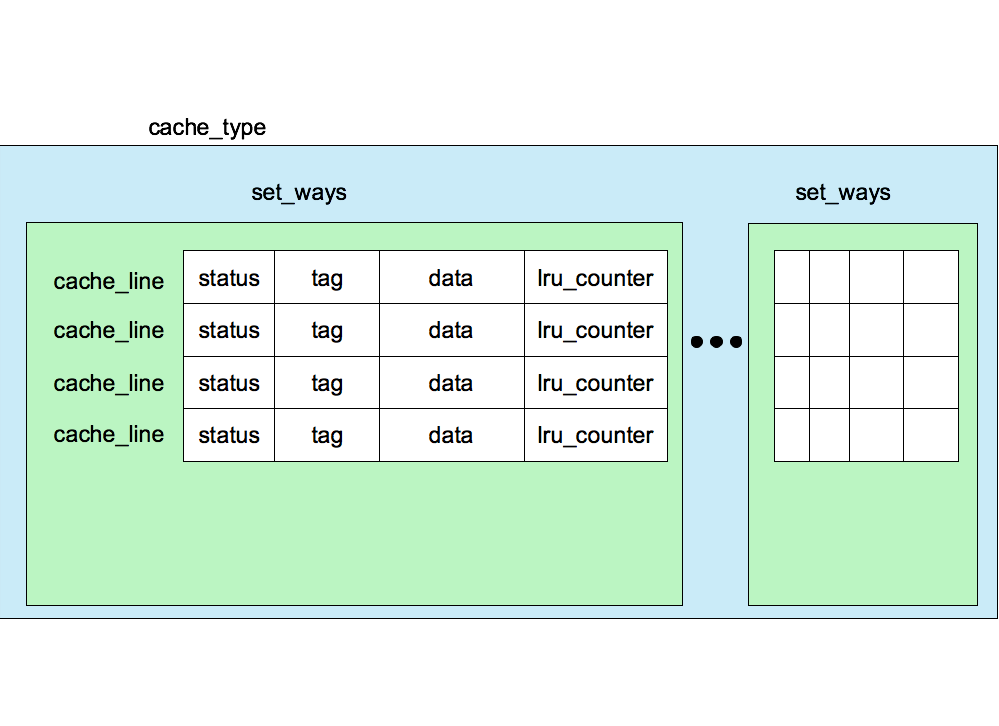
\includegraphics[width=\textwidth]{img/cacheType.png}
\caption{Schematizzazione delle strutture dati della cache}
\label{fig:c_type}
\end{figure}

In Fig. \ref{fig:c_type} \`e mostrata una schematizzazione delle strutture dati utilizzate all'interno della cache.

\section{Implementazione}

Il componente \texttt{Cache\_cmp} pu\`o concettualmente essere diviso in tre parti, ognuna delle quali si interfaccia rispettivamente con DLX, RAM e controllore di memoria.\\
Per questo motivo si \`e deciso di implementare il componente con 3 process indipendenti, i quali utilizzano segnali interni per sincronizzarsi, pi\`u un quarto processo che si occupa nello specifico di eseguire il rimpiazzamento delle linee.\\

\subsection{cache\_dlx}

Il process \texttt{cache\_dlx} si occupa dell'interfacciamento con il DLX eseguendo le operazioni di lettura e scrittura richieste attraverso gli opportuni segnali di controllo .
I compiti di questo process riguardano quindi i seguenti aspetti:
\begin{itemize}
  \item gestione della lettura di dati dalla cache;
  \item gestione della scrittura dei dati provenienti dal DLX nella cache;
  \item attivazione del meccanismo di rimpiazzamento di una linea;
  \item generazione del segnale di ready per il DLX;
\end{itemize}

La sensitivity list del processo comprende sia segnali esterni provenienti dal DLX, che segnali interni utilizzati per la sincronizzazione tra i diversi process.\\
In particolare sono preseti:
\begin{itemize}
  \item \texttt{ch\_memrd}: segnale esterno per una richiesta di lettura;
  \item \texttt{ch\_memwr}: segnale esterno per una richiesta di scrittura;
  \item \texttt{ch\_reset}: segnale esterno per effettuare il reset del contenuto della cache;
  \item \texttt{line\_ready}: segnale interno che indica il termine di un rimpiazzamento;
  \item \texttt{rdwr\_done}: segnale interno che indica, in caso di write-through, il completamento della scrittura in RAM.
\end{itemize}
 
I passi seguito durante una lettura sono:
\begin{enumerate}
  \item Lettura dell'indirizzo dal bus separando index, tag e offset;
  \item Verifica della presenza della linea in cache attraverso \texttt{get\_way()};
  \item In caso di MISS, attivazione del process per la politica di rimpiazzamento;
  \item Aggiornamento dei contatori attraverso \texttt{cache\_hit\_on()};
  \item Lettura del dato dalla cache ed emissione sul bus \texttt{ch\_bdata\_out}.
\end{enumerate}	

Per quanto riguarda invece la scrittura, si eseguono le seguenti operazioni:
\begin{enumerate}
  \item Lettura dell'indirizzo dal bus separando index, tag e offset; 
  \item Verifica della presenza della linea in cache attraverso \texttt{get\_way()};
  \item In caso di MISS, attivazione del process per la politica di rimpiazzamento;
  \item Scrittura del dato presente in \texttt{ch\_bdata\_in} nella cache;
  \item Aggiornamento dei contatori attraverso \texttt{cache\_hit\_on()};
  \item Aggiornamento del bit di stato ed eventuale write-through.
\end{enumerate}


%\lstset{caption=Codice VHDL del process \texttt{cache\_process}, label=DescriptiveLabel}

%\begin{lstlisting}
%Codice del process? Forse diventa un po' lungo...
%\end{lstlisting}


\subsection{cache\_ram}

Questo process si occupa dell'intefacciamento con la RAM. In particolare, attraverso segnali interni di controllo, possono essere attivati i meccanismi di scrittura e di lettura di un dato.\\

Durante la realizzazione si \`e ipotizzato che fosse disponibile un segnale di \texttt{ram\_ready} proveniente dall'esterno per indicare il completamento dell'operazione richiesta. Tale segnale \`e importante poich\`e le istruzioni all'interno di uno stesso process vengono eseguite in modo parallelo. Nel nostro caso non sarebbe quindi possibile emettere l'indirizzo per la RAM e leggere immediatamente di seguito i dati sul bus \texttt{ram\_data\_in}.\\

Nel nostro progetto si \`e supposto che tutti i componenti, compresa la RAM, eseguissero le operazioni in tempo nullo. Tuttavia il segnale \texttt{ram\_ready} diviene indispensabile nel caso in cui si decida di tenere in considerazione i ritardi introdotti da una RAM reale.


\subsection{cache\_snoop}

Il process \texttt{cache\_snoop} si attiva con il segnale esterno \texttt{ch\_eads} proveniente dal controllore di memoria e consente a quest'ultimo di operare sullo stato delle linee.\\
In particolare \`e possibile sapere se una determinata linea si trova in cache e se il suo stato \`e MESI\_M.\\
Tramite il segnale \texttt{ch\_inv} il controllore di memoria pu\`o inoltre forzare l'invalidazione di una particolare linea.\\

Il process \texttt{cache\_snoop} ha il seguente comportamento: se l'indirizzo richiesto non \`e presente in cache i segnali \texttt{ch\_hit} e \texttt{ch\_hitm} vengono portati al valore logico '0'. In caso contrario il comportamento varia in base allo stato della linea che contiene l'indirizzo:
\begin{itemize}
  \item stato MESI\_E: ch\_hit viene portato al valore '1' e la linea passa in stato MESI\_S;
  \item stato MESI\_S: ch\_hit viene portato al valore '1' e lo stato della linea resta invariato;
  \item stato MESI\_M: sia ch\_hit che ch\_hitm vengono portati al valore '1', viene forzata la scrittura della linea in RAM e il suo stato vien portato a MESI\_S.
\end{itemize}

Nel caso in cui il segnale ch\_inv sia attivo il comportamento resta invariato, ma lo stato della linea diventa sempre MESI\_I. 

\subsection{cache\_replace}

I meccasmi per il rimpiazzamento delle linee sono eseguiti dal process \texttt{cache\_replace}. In particolare questo process implementa la politica rimpiazzamento basata sui contatori, stabilendo di volta in volta quale linea rimpiazzare.\\

Il meccanismo non pu\`o eseguire tutte le operazioni in un unico ciclo, quindi per poter effettuare la sostituzione di una linea in cache con dei dati presenti in RAM \`e stato realizzato un \emph{sequencer} che compie le seguenti operazioni:
\begin{enumerate}
  \item determina la riga da sostituire;
  \item nel caso in cui tale linea sia in stato MESI\_M effettua il write-back sulla RAM;
  \item attende eventualmente il termine della scrittura;
  \item attiva il process per la lettura della nuova linea dalla RAM;
  \item attende il termine della lettura;
  \item comunica attraverso il segnale interno \texttt{line\_ready} che il rimpiazzamento \`e terminato.
\end{enumerate}

\subsection{Comunicazione tra processi}

I quattro processi si scambiano segnali che consentono la sincronizzazione delle operazioni da svolgere.\\

\begin{figure}[h!]
\centering
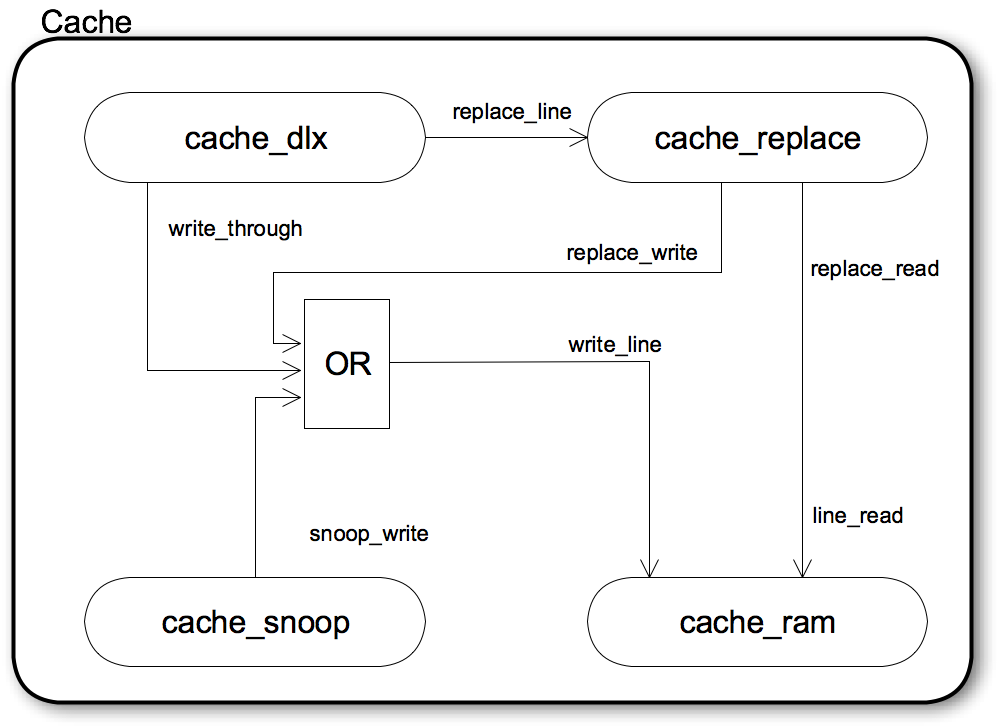
\includegraphics[width=\textwidth]{img/cache/collegamenti1.png}
\caption{Collegamenti tra processi}
\label{fig:colleg1}
\end{figure}

La Fig. \ref{fig:colleg1} mostra come sono collegati i seguenti segnali:
\begin{itemize}
  \item \texttt{replace\_line}: attiva il processo che gestisce il rimpiazzamento di una linea;
  \item \texttt{write\_through}: attiva la scrittura di una linea in stato \texttt{MESI\_S} in memoria RAM;
  \item \texttt{replace\_write}: attiva la scrittura di una linea da rimpiazzare in stato \texttt{MESI\_M} in memoria RAM;
  \item \texttt{snoop\_write}: attiva la scrittura di una linea in stato \texttt{MESI\_S} in memoria RAM in seguito ad uno snoop.
\end{itemize}

Ogni processo notifica il completamento dell'operazione richiesta attivando un opportuno segnale di ready, come mostrato in Fig. \ref{fig:colleg2}

\begin{figure}[h!]
\centering
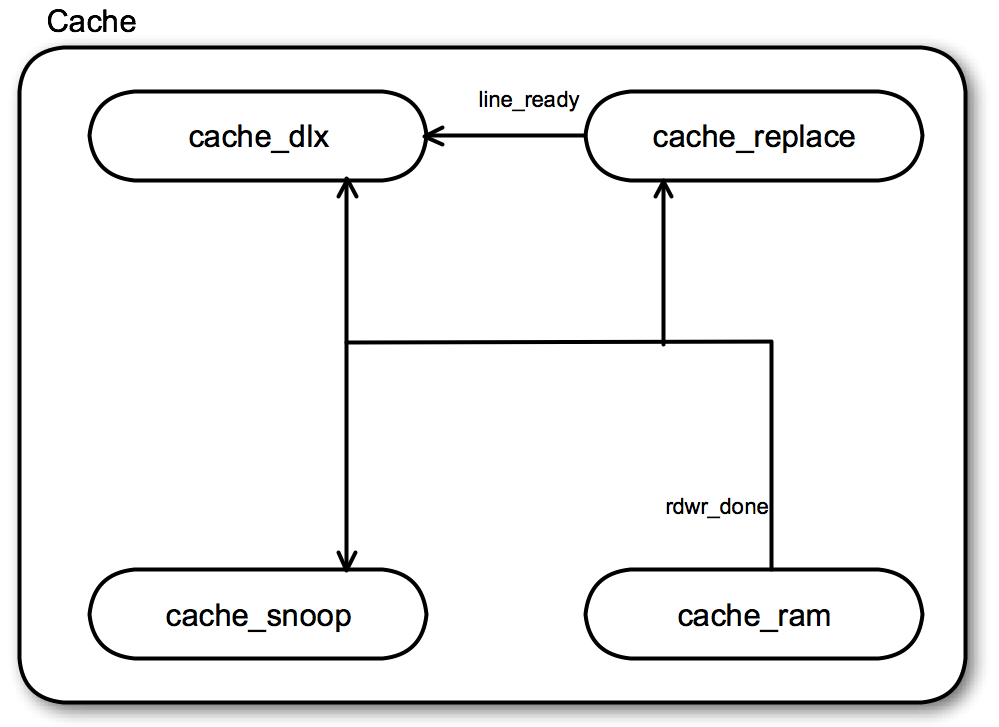
\includegraphics[width=\textwidth]{img/cache/collegamenti2.png}
\caption{Collegamenti tra processi}
\label{fig:colleg2}
\end{figure}


\section{Procedure interne}

Di seguito saranno brevemente descritte le procedure invocate all'interno dei diversi process.% \emph{(alcune non ci sono pi\`u e saranno da cavare)}


\subsection{cache\_replace\_line} %(selected\_way: out)}

Parametri di output:
\begin{itemize}
  \item selected\_way: via sulla quale \`e stato caricato il dato rimpiazzato
\end{itemize}

Descrizione:
\begin{enumerate}
  \item Individua la linea da rimpiazzare, cio\`e quella con \texttt{lru\_counter} massimo
  \item Controlla se la linea ha stato MESI\_M e in tal caso ne fa il write-back invocando \texttt{ram\_write()}
  \item Carica il nuovo blocco nella cache sovrascrivendo il vecchio
  \item Modifica il bit di stato in base al valore di WT\_WB
  \item Restituisce il numero della via sulla quale \`e presente il dato appena caricato
\end{enumerate}
		

\subsection{cache\_hit\_on} %(hit\_index: in, hit\_way: in)}

Parametri di input:
\begin{enumerate}
  \item \texttt{hit\_index}: indice al quale si \`e verificato l'hit
  \item \texttt{hit\_way}: via nella quale si \`e verificato l'hit
\end{enumerate}

Descrizione:

Applica la politica di invecchiamento aggiornando i contatori, in particolare:
\begin{enumerate}
  \item incrementa i contatori di valore pi\`u basso della via corrente specificata da \texttt{hit\_way}
  \item resetta il contatore della via corrente
\end{enumerate}	

\subsection{cache\_inv\_on} %(inv\_index: in, inv\_way: in)}

Parametri di input:
\begin{itemize}
  \item \texttt{inv\_index}: indice da invalidare
  \item \texttt{inv\_way}: via da invalidare
\end{itemize}

Descrizione:

Applica la politica di invecchiamento aggiornando i contatori, in particolare:
\begin{enumerate}
  \item decrementa i contatori di valore pi\`u alto della via corrente specificata da \texttt{inv\_way}
  \item porta al valore massimo il contatore della via corrente
\end{enumerate}	
	

\subsection{get\_way} %(index: in, tag: in, way: out) }

Parametri di input:
\begin{enumerate}
  \item \texttt{index}: indice
  \item \texttt{tag}: tag da controllare
\end{enumerate}	

Parametri di output:
\begin{itemize}
  \item \texttt{way}: via nella quale \`e presente il dato
\end{itemize}

Descrizione:	
\begin{enumerate}
  \item Verifica se il dato \`e in cache, cio\`e se esiste una linea con tag uguale a quello specificato il cui stato \`e diverso da \texttt{MESI\_I}
  \item Se il dato non \`e presente restituisce way = -1
  \item Se il dato \`e presente restituisce il numero della via
\end{enumerate}
	
	
%	
%\subsection{ram\_write} %(tag, index, way)}

%Parametri di input:
%\begin{itemize}
%  \item \texttt{tag}: tag della linea da scrivere
%  \item \texttt{index}: index della linea da scrivere
%  \item \texttt{way}: numero di via in cui si trova la linea da scrivere
%\end{itemize}

%Descrizione:
%	1. Costruisce l'indirizzo del blocco a partire da \texttt{tag} e \texttt{index}
%	2. Scrive i dati contenuti nel blocco sulla RAM


%\section{Diagrammi temporali}

%\section{Problematiche principali affrontate}

%(metteri anche tutti i problemi relativi al bus bidirezionale)\\

